%%%%%%%%%%%%  Generated using docx2latex.pythonanywhere.com  %%%%%%%%%%%%%%


\documentclass[a4paper,12pt]{report}

% Other options in place of 'report' are 1)article 2)book 3)letter
% Other options in place of 'a4paper' are 1)a5paper 2)b5paper 3)letterpaper 4)legalpaper 5)executivepaper


 %%%%%%%%%%%%  Include Packages  %%%%%%%%%%%%%%


\usepackage{amsmath}
\usepackage{latexsym}
\usepackage{amsfonts}
\usepackage{amssymb}
\usepackage{graphicx}
\usepackage{txfonts}
\usepackage{wasysym}
\usepackage{enumitem}
\usepackage{adjustbox}
\usepackage{ragged2e}
\usepackage{tabularx}
\usepackage{changepage}
\usepackage{setspace}
\usepackage{hhline}
\usepackage{multicol}
\usepackage{float}
\usepackage{multirow}
\usepackage{makecell}
\usepackage{fancyhdr}
\usepackage[toc,page]{appendix}
\usepackage[utf8]{inputenc}
\usepackage[T1]{fontenc}
\usepackage{hyperref}


 %%%%%%%%%%%%  Define Colors For Hyperlinks  %%%%%%%%%%%%%%


\hypersetup{
colorlinks=true,
linkcolor=blue,
filecolor=magenta,
urlcolor=cyan,
}
\urlstyle{same}


 %%%%%%%%%%%%  Set Depths for Sections  %%%%%%%%%%%%%%

% 1) Section
% 1.1) SubSection
% 1.1.1) SubSubSection
% 1.1.1.1) Paragraph
% 1.1.1.1.1) Subparagraph


\setcounter{tocdepth}{5}
\setcounter{secnumdepth}{5}


 %%%%%%%%%%%%  Set Page Margins  %%%%%%%%%%%%%%


\usepackage[a4paper,bindingoffset=0.2in,headsep=0.5cm,left=1.0in,right=1.0in,bottom=2cm,top=2cm,headheight=2cm]{geometry}
\everymath{\displaystyle}


 %%%%%%%%%%%%  Set Depths for Nested Lists created by \begin{enumerate}  %%%%%%%%%%%%%%


\setlistdepth{9}
\newlist{myEnumerate}{enumerate}{9}
	\setlist[myEnumerate,1]{label=\arabic*)}
	\setlist[myEnumerate,2]{label=\alph*)}
	\setlist[myEnumerate,3]{label=(\roman*)}
	\setlist[myEnumerate,4]{label=(\arabic*)}
	\setlist[myEnumerate,5]{label=(\Alph*)}
	\setlist[myEnumerate,6]{label=(\Roman*)}
	\setlist[myEnumerate,7]{label=\arabic*}
	\setlist[myEnumerate,8]{label=\alph*}
	\setlist[myEnumerate,9]{label=\roman*}

\renewlist{itemize}{itemize}{9}
	\setlist[itemize]{label=$\cdot$}
	\setlist[itemize,1]{label=\textbullet}
	\setlist[itemize,2]{label=$\circ$}
	\setlist[itemize,3]{label=$\ast$}
	\setlist[itemize,4]{label=$\dagger$}
	\setlist[itemize,5]{label=$\triangleright$}
	\setlist[itemize,6]{label=$\bigstar$}
	\setlist[itemize,7]{label=$\blacklozenge$}
	\setlist[itemize,8]{label=$\prime$}



 %%%%%%%%%%%%  Header here  %%%%%%%%%%%%%%


\pagestyle{fancy}
\fancyhf{}


 %%%%%%%%%%%%  Footer here  %%%%%%%%%%%%%%




 %%%%%%%%%%%%  Print Page Numbers  %%%%%%%%%%%%%%


\rfoot{\thepage}


 %%%%%%%%%%%%  This sets linespacing (verticle gap between Lines) Default=1 %%%%%%%%%%%%%%


\setstretch{1.08}


 %%%%%%%%%%%%  Document Code starts here %%%%%%%%%%%%%%


\begin{document}
\sloppy
\begin{center}{\fontsize{14pt}{14pt}\selectfont \textbf{LISTS} \\}\end{center} \par
\noindent 
{\fontsize{14pt}{14pt}\selectfont Struktur data yang paling dasar dengan Python adalah urutannya. Setiap elemen berurutan diberi nomor - posisinya atau indeksnya. Indeks pertama adalah nol, indeks kedua adalah satu, dan seterusnya. \\} \par
\vspace{14pt}
\noindent 
{\fontsize{14pt}{14pt}\selectfont Python memiliki enam jenis urutan built-in, namun yang paling umum adalah daftar dan tupel, yang akan kami lihat di tutorial ini. \\} \par
\noindent 
{\fontsize{14pt}{14pt}\selectfont Ada beberapa hal yang dapat Anda lakukan dengan semua tipe urutan. Operasi ini meliputi pengindeksan, pengiris, penambahan, perbanyak, dan pengecekan keanggotaan. Selain itu, Python memiliki fungsi built-in untuk menemukan panjang urutan dan untuk menemukan elemen terbesar dan terkecilnya. \\} \par
\vspace{14pt}
\noindent 
{\fontsize{14pt}{14pt}\selectfont Daftar Python \\} \par
\vspace{14pt}
\noindent 
{\fontsize{14pt}{14pt}\selectfont Daftar ini adalah datatype paling serbaguna yang tersedia dengan Python yang dapat ditulis sebagai daftar nilai yang dipisahkan koma (item) antara tanda kurung siku. Hal penting tentang daftar adalah item dalam daftar tidak perlu jenis yang sama. \\} \par
\noindent 
{\fontsize{14pt}{14pt}\selectfont Membuat daftar sesederhana memasukkan berbagai nilai yang dipisahkan koma di antara tanda kurung siku. Misalnya - \\} \par
\noindent 
\vspace{14pt}
\noindent 
{\fontsize{14pt}{14pt}\selectfont list1 = ['physics', 'chemistry', 1997, 2000]; \\} \par
\noindent 
{\fontsize{14pt}{14pt}\selectfont list2 = [1, 2, 3, 4, 5 ]; \\} \par
\noindent 
{\fontsize{14pt}{14pt}\selectfont list3 = ["a", "b", "c", "d"] \\} \par
\noindent 
{\fontsize{14pt}{14pt}\selectfont Serupa dengan indeks string, daftar indeks mulai dari 0, dan daftar dapat diiris, digabungkan dan seterusnya. \\} \par
\noindent 
{\fontsize{14pt}{14pt}\selectfont Mengakses Nilai dalam Daftar \\} \par
\noindent 
{\fontsize{14pt}{14pt}\selectfont Untuk mengakses nilai dalam daftar, gunakan tanda kurung siku untuk mengiris beserta indeks atau indeks untuk mendapatkan nilai yang tersedia pada indeks tersebut. Misalnya - \\} \par
\vspace{14pt}
\noindent 
{\fontsize{14pt}{14pt}\selectfont  $  \#  $! / Usr / bin / python \\} \par
\vspace{14pt}
\noindent 
{\fontsize{14pt}{14pt}\selectfont List1 = ['fisika', 'kimia', 1997, 2000]; \\} \par
\noindent 
{\fontsize{14pt}{14pt}\selectfont List2 = [1, 2, 3, 4, 5, 6, 7]; \\} \par
\vspace{14pt}
\noindent 
{\fontsize{14pt}{14pt}\selectfont Cetak "list1 [0]:", list1 [0] \\} \par
\noindent 
{\fontsize{14pt}{14pt}\selectfont Cetak "list2 [1: 5]:", list2 [1: 5] \\} \par
\vspace{14pt}
\noindent 
{\fontsize{14pt}{14pt}\selectfont Bila kode diatas dieksekusi, maka menghasilkan hasil sebagai berikut - \\} \par
\vspace{14pt}
\noindent 
{\fontsize{14pt}{14pt}\selectfont List1 [0]: fisika \\} \par
\noindent 
{\fontsize{14pt}{14pt}\selectfont List2 [1: 5]: [2, 3, 4, 5] \\} \par
\vspace{14pt}
\noindent 
{\fontsize{14pt}{14pt}\selectfont Memperbarui Daftar \\} \par
\vspace{14pt}
\noindent 
{\fontsize{14pt}{14pt}\selectfont Anda dapat memperbarui satu atau beberapa elemen daftar dengan memberikan potongan di sisi kiri operator penugasan, dan Anda dapat menambahkan ke elemen dalam daftar dengan metode append (). Misalnya - \\} \par
\vspace{14pt}
\noindent 
{\fontsize{14pt}{14pt}\selectfont  $  \#  $! / Usr / bin / python \\} \par
\noindent 
\vspace{14pt}
\noindent 
{\fontsize{14pt}{14pt}\selectfont list = ['physics', 'chemistry', 1997, 2000]; \\} \par
\noindent 
\vspace{14pt}
\noindent 
{\fontsize{14pt}{14pt}\selectfont print "Value available at index 2 : " \\} \par
\noindent 
{\fontsize{14pt}{14pt}\selectfont print list[2] \\} \par
\noindent 
{\fontsize{14pt}{14pt}\selectfont list[2] = 2001; \\} \par
\noindent 
{\fontsize{14pt}{14pt}\selectfont print "New value available at index 2 : " \\} \par
\noindent 
{\fontsize{14pt}{14pt}\selectfont print list[2] \\} \par
\noindent 
{\fontsize{14pt}{14pt}\selectfont Catatan: append () metode dibahas di bagian selanjutnya. \\} \par
\vspace{14pt}
\noindent 
{\fontsize{14pt}{14pt}\selectfont Bila kode diatas dieksekusi, maka menghasilkan hasil sebagai berikut - \\} \par
\noindent 
{\fontsize{14pt}{14pt}\selectfont Nilai tersedia di indeks 2: \\} \par
\vspace{14pt}
\noindent 
{\fontsize{14pt}{14pt}\selectfont 1997 \\} \par
\vspace{14pt}
\noindent 
{\fontsize{14pt}{14pt}\selectfont Nilai baru tersedia di indeks 2: \\} \par
\vspace{14pt}
\noindent 
{\fontsize{14pt}{14pt}\selectfont 2001 \\} \par
\vspace{14pt}
\noindent 
{\fontsize{14pt}{14pt}\selectfont Hapus Daftar Elemen \\} \par
\vspace{14pt}
\noindent 
{\fontsize{14pt}{14pt}\selectfont Untuk menghapus elemen daftar, Anda dapat menggunakan salah satu pernyataan del jika Anda tahu persis elemen yang Anda hapus atau metode hapus () jika Anda tidak mengetahuinya. Misalnya - \\} \par
\vspace{14pt}
\noindent 
{\fontsize{14pt}{14pt}\selectfont  $  \#  $! / Usr / bin / python \\} \par
\vspace{14pt}
\noindent 
{\fontsize{14pt}{14pt}\selectfont List1 = ['fisika', 'kimia', 1997, 2000]; \\} \par
\vspace{14pt}
\noindent 
{\fontsize{14pt}{14pt}\selectfont Daftar cetak1 \\} \par
\vspace{14pt}
\noindent 
{\fontsize{14pt}{14pt}\selectfont Del list1 [2]; \\} \par
\vspace{14pt}
\noindent 
{\fontsize{14pt}{14pt}\selectfont Cetak "Setelah menghapus nilai pada indeks 2:" \\} \par
\vspace{14pt}
\noindent 
{\fontsize{14pt}{14pt}\selectfont Daftar cetak1 \\} \par
\noindent 
{\fontsize{14pt}{14pt}\selectfont Bila kode diatas dieksekusi, maka menghasilkan hasil sebagai berikut - \\} \par
\noindent 
{\fontsize{14pt}{14pt}\selectfont ['Fisika', 'kimia', 1997, 2000] \\} \par
\noindent 
{\fontsize{14pt}{14pt}\selectfont Setelah menghapus nilai pada indeks 2: \\} \par
\noindent 
{\fontsize{14pt}{14pt}\selectfont ['Fisika', 'kimia', 2000] \\} \par
\noindent 
{\fontsize{14pt}{14pt}\selectfont Catatan: hapus () metode dibahas di bagian selanjutnya. \\} \par
\noindent 
{\fontsize{14pt}{14pt}\selectfont Operasi Daftar Dasar \\} \par
\noindent 
{\fontsize{14pt}{14pt}\selectfont Daftar merespons operator + dan * seperti string; Mereka berarti penggabungan dan pengulangan di sini juga, kecuali hasilnya adalah daftar baru, bukan string. \\} \par
\noindent 
{\fontsize{14pt}{14pt}\selectfont Sebenarnya, daftar merespons semua operasi urutan umum yang kami gunakan pada senar di bab sebelumnya. \\} \par


 %%%%%%%%%%%%  Table No:1 Here %%%%%%%%%%%%%%


\begin{table}[H]
\centering
\begin{adjustbox}{width=\textwidth}
\begin{tabular}{ p{1.7in}p{1.69in}p{1.7in} }
\hhline{---}
\multicolumn{1}{|p{1.7in}}{\Centering \textbf{Python Expression}} & \multicolumn{1}{|p{1.69in}}{\Centering \textbf{Results }} & \multicolumn{1}{|p{1.7in}|}{\Centering \textbf{Description}} & \hhline{---}
\multicolumn{1}{|p{1.7in}}{len([1, 2, 3])} & \multicolumn{1}{|p{1.69in}}{3} & \multicolumn{1}{|p{1.7in}|}{Length} & \hhline{---}
\multicolumn{1}{|p{1.7in}}{[1, 2, 3] + [4, 5, 6]} & \multicolumn{1}{|p{1.69in}}{[1, 2, 3, 4, 5, 6]} & \multicolumn{1}{|p{1.7in}|}{Concatenation} & \hhline{---}
\multicolumn{1}{|p{1.7in}}{['Hi!'] * 4} & \multicolumn{1}{|p{1.69in}}{['Hi!', 'Hi!', 'Hi!', 'Hi!']} & \multicolumn{1}{|p{1.7in}|}{Repetition} & \hhline{---}
\multicolumn{1}{|p{1.7in}}{3 in [1, 2, 3]} & \multicolumn{1}{|p{1.69in}}{True} & \multicolumn{1}{|p{1.7in}|}{Membership} & \hhline{---}
\multicolumn{1}{|p{1.7in}}{for x in [1, 2, 3]: print x,} & \multicolumn{1}{|p{1.69in}}{1 2 3} & \multicolumn{1}{|p{1.7in}|}{Iteration} & \hline
\end{tabular}
\end{adjustbox}
\end{table}


 %%%%%%%%%%%%  Table No:1 Ends Here %%%%%%%%%%%%%%


\vspace{14pt}
\noindent 
{\fontsize{14pt}{14pt}\selectfont Indexing, Slicing, dan Matrixes \\} \par
\noindent 
{\fontsize{14pt}{14pt}\selectfont Karena daftar adalah urutan, pengindeksan dan pengiris bekerja dengan cara yang sama untuk daftar seperti yang mereka lakukan untuk string. \\} \par
\noindent 
{\fontsize{14pt}{14pt}\selectfont Dengan asumsi masukan berikut - \\} \par
\noindent 
{\fontsize{14pt}{14pt}\selectfont L = ['spam', 'Spam', 'SPAM!'] \\} \par
\noindent 
{\fontsize{14pt}{14pt}\selectfont  $  $ \\} \par


 %%%%%%%%%%%%  Table No:2 Here %%%%%%%%%%%%%%


\begin{table}[H]
\centering
\begin{adjustbox}{width=\textwidth}
\begin{tabular}{ p{2.09in}p{2.08in}p{2.09in} }
\hhline{---}
\multicolumn{1}{|p{2.09in}}{\Centering \textbf{Python Expression}} & \multicolumn{1}{|p{2.08in}}{\Centering \textbf{Results }} & \multicolumn{1}{|p{2.09in}|}{\Centering \textbf{Description}} & \hhline{---}
\multicolumn{1}{|p{2.09in}}{L[2]} & \multicolumn{1}{|p{2.08in}}{'SPAM!'} & \multicolumn{1}{|p{2.09in}|}{Offsets start at zero} & \hhline{---}
\multicolumn{1}{|p{2.09in}}{L[-2]} & \multicolumn{1}{|p{2.08in}}{'Spam'} & \multicolumn{1}{|p{2.09in}|}{Negative: count from the right} & \hhline{---}
\multicolumn{1}{|p{2.09in}}{L[1:]} & \multicolumn{1}{|p{2.08in}}{['Spam', 'SPAM!']} & \multicolumn{1}{|p{2.09in}|}{Slicing fetches sections} & \hline
\end{tabular}
\end{adjustbox}
\end{table}


 %%%%%%%%%%%%  Table No:2 Ends Here %%%%%%%%%%%%%%


\noindent 
{\fontsize{14pt}{14pt}\selectfont \textbf{Built-in List Functions  $  \&  $ Methods:} \\} \par
\noindent 
{\fontsize{14pt}{14pt}\selectfont Python includes the following list functions – \\} \par
\vspace{14pt}


 %%%%%%%%%%%%  Table No:3 Here %%%%%%%%%%%%%%


\begin{table}[H]
\centering
\begin{adjustbox}{width=\textwidth}
\begin{tabular}{ p{0.3in}p{5.15in} }
\hhline{--}
\multicolumn{1}{|p{0.3in}}{\Centering \textbf{SN}} & \multicolumn{1}{|p{5.15in}|}{\Centering \textbf{Function with Description}} & \hhline{--}
\multicolumn{1}{|p{0.3in}}{1} & \multicolumn{1}{|p{5.15in}|}{\href{https://www.tutorialspoint.com/python/list $  \_  $cmp.htm}{cmp(list1, list2)}
Compares elements of both lists.} & \hhline{--}
\multicolumn{1}{|p{0.3in}}{2} & \multicolumn{1}{|p{5.15in}|}{\href{https://www.tutorialspoint.com/python/list $  \_  $len.htm}{len(list)}
Gives the total length of the list.} & \hhline{--}
\multicolumn{1}{|p{0.3in}}{3} & \multicolumn{1}{|p{5.15in}|}{\href{https://www.tutorialspoint.com/python/list $  \_  $max.htm}{max(list)}
Returns item from the list with max value.} & \hhline{--}
\multicolumn{1}{|p{0.3in}}{4} & \multicolumn{1}{|p{5.15in}|}{\href{https://www.tutorialspoint.com/python/list $  \_  $min.htm}{min(list)}
Returns item from the list with min value.} & \hhline{--}
\multicolumn{1}{|p{0.3in}}{5} & \multicolumn{1}{|p{5.15in}|}{\href{https://www.tutorialspoint.com/python/list $  \_  $list.htm}{list(seq)}
Converts a tuple into list.} & \hline
\end{tabular}
\end{adjustbox}
\end{table}


 %%%%%%%%%%%%  Table No:3 Ends Here %%%%%%%%%%%%%%


\noindent 
{\fontsize{14pt}{14pt}\selectfont Python includes following list methods \\} \par


 %%%%%%%%%%%%  Table No:4 Here %%%%%%%%%%%%%%


\begin{table}[H]
\centering
\begin{adjustbox}{width=\textwidth}
\begin{tabular}{ p{0.3in}p{5.15in} }
\hhline{--}
\multicolumn{1}{|p{0.3in}}{\Centering \textbf{SN}} & \multicolumn{1}{|p{5.15in}|}{\Centering \textbf{Methods with Description}} & \hhline{--}
\multicolumn{1}{|p{0.3in}}{1} & \multicolumn{1}{|p{5.15in}|}{\href{https://www.tutorialspoint.com/python/list $  \_  $append.htm}{list.append(obj)}
Appends object obj to list} & \hhline{--}
\multicolumn{1}{|p{0.3in}}{2} & \multicolumn{1}{|p{5.15in}|}{\href{https://www.tutorialspoint.com/python/list $  \_  $count.htm}{list.count(obj)}
Returns count of how many times obj occurs in list} & \hhline{--}
\multicolumn{1}{|p{0.3in}}{3} & \multicolumn{1}{|p{5.15in}|}{\href{https://www.tutorialspoint.com/python/list $  \_  $extend.htm}{list.extend(seq)}
Appends the contents of seq to list} & \hhline{--}
\multicolumn{1}{|p{0.3in}}{4} & \multicolumn{1}{|p{5.15in}|}{\href{https://www.tutorialspoint.com/python/list $  \_  $index.htm}{list.index(obj)}
Returns the lowest index in list that obj appears} & \hhline{--}
\multicolumn{1}{|p{0.3in}}{5} & \multicolumn{1}{|p{5.15in}|}{\href{https://www.tutorialspoint.com/python/list $  \_  $insert.htm}{list.insert(index, obj)}
Inserts object obj into list at offset index} & \hhline{--}
\multicolumn{1}{|p{0.3in}}{6} & \multicolumn{1}{|p{5.15in}|}{\href{https://www.tutorialspoint.com/python/list $  \_  $pop.htm}{list.pop(obj=list[-1])}
Removes and returns last object or obj from list} & \hhline{--}
\multicolumn{1}{|p{0.3in}}{7} & \multicolumn{1}{|p{5.15in}|}{\href{https://www.tutorialspoint.com/python/list $  \_  $remove.htm}{list.remove(obj)}
Removes object obj from list} & \hhline{--}
\multicolumn{1}{|p{0.3in}}{8} & \multicolumn{1}{|p{5.15in}|}{\href{https://www.tutorialspoint.com/python/list $  \_  $reverse.htm}{list.reverse()}
Reverses objects of list in place} & \hhline{--}
\multicolumn{1}{|p{0.3in}}{9} & \multicolumn{1}{|p{5.15in}|}{\href{https://www.tutorialspoint.com/python/list $  \_  $sort.htm}{list.sort([func])}
Sorts objects of list, use compare func if given} & \hline
\end{tabular}
\end{adjustbox}
\end{table}


 %%%%%%%%%%%%  Table No:4 Ends Here %%%%%%%%%%%%%%


\vspace{14pt}
\noindent 
Python memiliki tipe daftar built-in yang hebat dengan nama "daftar". Daftar literal ditulis dalam tanda kurung siku []. Daftar bekerja sama dengan senar - gunakan fungsi len () dan tanda kurung siku [] untuk mengakses data, dengan elemen pertama di indeks 0. (Lihat daftar dokumen python.org resmi). \par
\noindent 
\vspace{10pt}
\noindent 
{\fontsize{10pt}{10pt}\selectfont  $  $ $  $Warna = ['merah', 'biru', 'hijau']} \par
\noindent 
 $  $ $  $cetak warna [0]  $  \#  $ $  \#  $ merah \par
\noindent 
 $  $ $  $cetak warna [2]  $  \#  $ $  \#  $ hijau \par
\noindent 
 $  $ $  $Cetak len (warna)  $  \#  $ $  \#  $ 3 \par
\noindent 
\vspace{12pt}
\noindent 
\vspace{12pt}
\noindent 


 %%%%%%%%%%%%  Figure/Image No:1 here %%%%%%%%%%%%%%


\begin{figure}[H]
\begin{center}
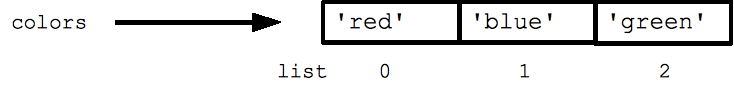
\includegraphics[width=6.26in,height=0.88in]{./uploads_new/LISTS.docx_DIR/media/image1.png}
\end{center}
\end{figure}


 %%%%%%%%%%%%  Figure/Image No:1 Ends Here %%%%%%%%%%%%%%


{\fontsize{14pt}{14pt}\selectfont  \\}\vspace{14pt}
\noindent 
Tugas dengan = daftar tidak membuat salinan. Sebagai gantinya, tugas membuat kedua variabel menunjuk ke satu daftar di memori. \par
\noindent 
\vspace{10pt}
\noindent 
{\fontsize{10pt}{10pt}\selectfont  $  $ $  $B = warna  $  \#  $ $  \#  $ Tidak menyalin daftar} \par
\noindent 


 %%%%%%%%%%%%  Figure/Image No:2 here %%%%%%%%%%%%%%


\begin{figure}[H]
\begin{center}
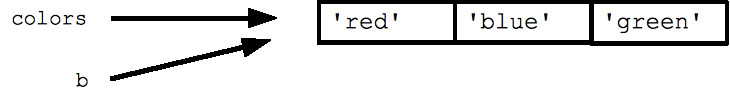
\includegraphics[width=6.27in,height=0.96in]{./uploads_new/LISTS.docx_DIR/media/image2.png}
\end{center}
\end{figure}


 %%%%%%%%%%%%  Figure/Image No:2 Ends Here %%%%%%%%%%%%%%


{\fontsize{14pt}{14pt}\selectfont  \\}\vspace{14pt}
\noindent 
"Daftar kosong" hanyalah sepasang kurung kosong []. '+' Bekerja untuk menambahkan dua daftar, jadi [1, 2] + [3, 4] menghasilkan [1, 2, 3, 4] (ini sama seperti + dengan string). \par
\noindent 
FOR dan IN \par
\vspace{12pt}
\noindent 
Python's * untuk * dan * in * constructs sangat berguna, dan penggunaan pertama dari yang akan kita lihat adalah dengan daftar. * Untuk * membangun - untuk daftar var - adalah cara mudah untuk melihat setiap elemen dalam daftar (atau koleksi lainnya). Jangan menambah atau menghapus dari daftar selama iterasi. \par
\vspace{12pt}
\noindent 
 $  $ $  $kotak = [1, 4, 9, 16] \par
\noindent 
 $  $ $  $Jumlah = 0 \par
\noindent 
 $  $ $  $Untuk num dalam kotak: \par
\noindent 
 $  $ $  $ $  $ $  $Jumlah + = num \par
\noindent 
 $  $ $  $Jumlah cetak \par
\vspace{14pt}
\noindent 
Jika Anda tahu hal macam apa yang ada dalam daftar, gunakan nama variabel dalam lingkaran yang menangkap informasi seperti "num", atau "name", atau "url". Karena kode python tidak memiliki sintaks lain untuk mengingatkan Anda tentang tipe, nama variabel Anda adalah cara kunci bagi Anda untuk tetap mempertahankan apa yang sedang terjadi. \par
\vspace{12pt}
\noindent 
* Dalam * membangun sendiri adalah cara mudah untuk menguji apakah sebuah elemen muncul dalam daftar (atau koleksi lainnya) - nilai dalam koleksi - tes jika nilainya ada dalam koleksi, mengembalikan True / False. \par
\vspace{12pt}
\noindent 
 $  $ $  $Daftar = ['larry', 'curly', 'moe'] \par
\noindent 
 $  $ $  $jika 'keriting' dalam daftar: \par
\noindent 
 $  $ $  $ $  $ $  $Cetak 'yay' \par
\vspace{12pt}
\noindent 
The for / in constructs sangat umum digunakan pada kode Python dan bekerja pada tipe data selain list, jadi sebaiknya hafalkan sintaksnya. Anda mungkin memiliki kebiasaan dari bahasa lain di mana Anda memulai pengulangan manual melalui koleksi, dengan Python yang seharusnya Anda gunakan untuk / in. \par
\vspace{12pt}
\noindent 
Anda juga dapat menggunakannya untuk / dalam mengerjakan sebuah string. String bertindak seperti daftar karakternya, jadi untuk ch di s: print ch mencetak semua karakter dalam sebuah string. \par
\noindent 
Jarak \par
\vspace{12pt}
\noindent 
Fungsi range (n) menghasilkan angka 0, 1, ... n-1, dan range (a, b) mengembalikan a, a + 1, ... b-1 - sampai tapi tidak termasuk angka terakhir . Kombinasi fungsi for-loop dan range () memungkinkan Anda membuat numerik tradisional untuk loop: \par
\vspace{12pt}
\vspace{12pt}
\noindent 
 $  \#  $ $  \#  $ print the numbers from 0 through 99\vspace{\baselineskip}
 $  $ for i in range(100):\vspace{\baselineskip}
 $  $  $  $ print i \par
\vspace{14pt}
\noindent 
{\fontsize{14pt}{14pt}\selectfont Ada varian xrange () yang menghindari biaya membangun keseluruhan daftar untuk kasus sensitif kinerja (dalam Python 3000, range () akan memiliki perilaku kinerja yang baik dan Anda dapat melupakan xrange ()). \\} \par
\noindent 
{\fontsize{14pt}{14pt}\selectfont Sementara Loop \\} \par
\vspace{14pt}
\noindent 
{\fontsize{14pt}{14pt}\selectfont Python juga memiliki standar while-loop, dan * break * dan * continue * statements bekerja seperti di C ++ dan Java, mengubah jalannya loop terdalam. Di atas untuk / dalam loop memecahkan kasus umum iterasi pada setiap elemen dalam daftar, namun loop sementara memberi Anda kontrol penuh atas angka indeks. Berikut adalah loop sementara yang mengakses setiap elemen ke-3 dalam daftar: \\} \par
\vspace{12pt}
\noindent 
 $  $ $  $ $  \#  $ $  \#  $ Mengakses setiap elemen ke-3 dalam daftar \par
\noindent 
 $  $ $  $I = 0 \par
\noindent 
 $  $ $  $sementara i <len (a): \par
\noindent 
 $  $ $  $ $  $ $  $cetak sebuah [i] \par
\noindent 
 $  $ $  $ $  $ $  $i = i + 3 \par
\noindent 
{\fontsize{14pt}{14pt}\selectfont Daftar metode \\} \par
\vspace{14pt}
\noindent 
{\fontsize{14pt}{14pt}\selectfont Berikut adalah beberapa metode daftar umum lainnya. \\} \par
\vspace{14pt}
\noindent 
{\fontsize{14pt}{14pt}\selectfont  $  $ $  $ $  $ $  $List.append (elem) - menambahkan satu elemen ke akhir daftar. Kesalahan umum: tidak mengembalikan daftar baru, cukup modifikasi yang asli. \\} \par
\noindent 
{\fontsize{14pt}{14pt}\selectfont  $  $ $  $ $  $ $  $List.insert (indeks, elem) - memasukkan elemen pada indeks yang diberikan, menggeser elemen ke kanan. \\} \par
\noindent 
{\fontsize{14pt}{14pt}\selectfont  $  $ $  $ $  $ $  $List.extend (list2) menambahkan elemen dalam list2 ke akhir daftar. Menggunakan + atau + = pada daftar sama dengan menggunakan extend (). \\} \par
\noindent 
{\fontsize{14pt}{14pt}\selectfont  $  $ $  $ $  $ $  $List.index (elem) - mencari elemen yang diberikan dari awal daftar dan mengembalikan indeksnya. Melempar ValueError jika elemen tidak muncul (gunakan "in" untuk memeriksa tanpa ValueError). \\} \par
\noindent 
{\fontsize{14pt}{14pt}\selectfont  $  $ $  $ $  $ $  $List.remove (elem) - mencari instance pertama dari elemen yang diberikan dan menghapusnya (melempar ValueError jika tidak ada) \\} \par
\noindent 
{\fontsize{14pt}{14pt}\selectfont  $  $ $  $ $  $ $  $List.sort () - menyusun daftar di tempat (tidak mengembalikannya). (Fungsi yang diurutkan () yang ditunjukkan di bawah ini lebih diutamakan.) \\} \par
\noindent 
{\fontsize{14pt}{14pt}\selectfont  $  $ $  $ $  $ $  $List.reverse () - membalik daftar di tempat (tidak mengembalikannya) \\} \par
\noindent 
{\fontsize{14pt}{14pt}\selectfont  $  $ $  $ $  $ $  $List.pop (index) - menghapus dan mengembalikan elemen pada indeks yang diberikan. Mengembalikan elemen paling kanan jika indeks dihilangkan (kira-kira kebalikan dari append ()). \\} \par
\vspace{14pt}
\noindent 
{\fontsize{14pt}{14pt}\selectfont Perhatikan bahwa ini adalah * metode * pada daftar objek, sedangkan len () adalah fungsi yang mengambil daftar (atau string atau apapun) sebagai argumen. \\} \par
\vspace{14pt}
\vspace{14pt}
\noindent 
Daftar = ['larry', 'curly', 'moe'] \par
\noindent 
 $  $ $  $List.append ('shemp')  $  \#  $ $  \#  $ append elem di akhir \par
\noindent 
 $  $ $  $List.insert (0, 'xxx')  $  \#  $ $  \#  $ masukkan elem pada indeks 0 \par
\noindent 
 $  $ $  $list.extend (['yyy', 'zzz'])  $  \#  $ $  \#  $ tambahkan daftar elems at end \par
\noindent 
 $  $ $  $daftar cetak  $  \#  $ $  \#  $ ['xxx', 'larry', 'curly', 'moe', 'shemp', 'yyy', 'zzz'] \par
\noindent 
 $  $ $  $Print list.index ('keriting')  $  \#  $ $  \#  $ 2 \par
\vspace{12pt}
\noindent 
 $  $ $  $List.remove ('curly')  $  \#  $ $  \#  $ cari dan hapus elemen itu \par
\noindent 
 $  $ $  $List.pop (1)  $  \#  $ $  \#  $ menghapus dan mengembalikan 'larry' \par
\noindent 
 $  $ $  $daftar cetak  $  \#  $ $  \#  $ ['xxx', 'moe', 'shemp', 'yyy', 'zzz'] \par
\vspace{12pt}
\noindent 
Kesalahan umum: perhatikan bahwa metode di atas tidak * mengembalikan * daftar yang dimodifikasi, mereka hanya memodifikasi daftar aslinya. \par
\vspace{12pt}
\noindent 
 $  $ $  $Daftar = [1, 2, 3] \par
\noindent 
 $  $ $  $Print list.append (4)  $  \#  $ $  \#  $ TIDAK, tidak bekerja, append () return Tidak ada \par
\noindent 
 $  $ $  $ $  \#  $ $  \#  $ Pola yang benar: \par
\noindent 
 $  $ $  $List.append (4) \par
\noindent 
 $  $ $  $Daftar cetak  $  \#  $ $  \#  $ [1, 2, 3, 4] \par
\noindent 
st Build Up \par
\vspace{12pt}
\noindent 
Salah satu pola yang umum adalah dengan memulai daftar daftar kosong [], lalu gunakan append () atau extend () untuk menambahkan elemen ke dalamnya: \par
\vspace{12pt}
\noindent 
 $  $ $  $List = []  $  \#  $ $  \#  $ Mulai sebagai daftar kosong \par
\noindent 
 $  $ $  $List.append ('a')  $  \#  $ $  \#  $ Gunakan append () untuk menambahkan elemen \par
\noindent 
 $  $ $  $List.append ('b') \par
\vspace{12pt}
\noindent 
Daftar irisan \par
\vspace{12pt}
\noindent 
Slice bekerja pada daftar seperti halnya senar, dan juga dapat digunakan untuk mengubah sub-bagian daftar. \par
\vspace{12pt}
\noindent 
 $  $ $  $Daftar = ['a', 'b', 'c', 'd'] \par
\noindent 
 $  $ $  $Daftar cetak [1: -1]  $  \#  $ $  \#  $ ['b', 'c'] \par
\noindent 
 $  $ $  $Daftar [0: 2] = 'z'  $  \#  $ $  \#  $ ganti ['a', 'b'] dengan ['z'] \par
\noindent 
 $  $ $  $Daftar cetak  $  \#  $ $  \#  $ ['z', 'c', 'd'] \par
\noindent 
Tipe data daftar memiliki beberapa metode lagi. Berikut adalah semua metode daftar objek: \par
\vspace{12pt}
\noindent 
List.append (x) \par
\vspace{12pt}
\noindent 
 $  $ $  $ $  $ $  $Tambahkan item ke bagian akhir daftar. Setara dengan [len (a):] = [x]. \par
\vspace{12pt}
\noindent 
list.extend (iterable) \par
\vspace{12pt}
\noindent 
 $  $ $  $ $  $ $  $Perluas daftar dengan menambahkan semua item dari iterable. Setara dengan [len (a):] = iterable. \par
\vspace{12pt}
\noindent 
list.insert (i, x) \par
\vspace{12pt}
\noindent 
 $  $ $  $ $  $ $  $Masukkan item pada posisi tertentu. Argumen pertama adalah indeks dari elemen yang sebelum dimasukkan, jadi a.insert (0, x) memasukkan di bagian depan daftar, dan a.insert (len (a), x) setara dengan a.append ( x). \par
\vspace{12pt}
\noindent 
List.remove (x) \par
\vspace{12pt}
\noindent 
 $  $ $  $ $  $ $  $Hapus item pertama dari daftar yang nilainya x. Ini adalah kesalahan jika tidak ada item seperti itu. \par
\vspace{12pt}
\noindent 
List.pop ([i]) \par
\vspace{12pt}
\noindent 
 $  $ $  $ $  $ $  $Hapus item pada posisi yang diberikan dalam daftar, dan kembalikan. Jika tidak ada indeks yang ditentukan, a.pop () menghapus dan mengembalikan item terakhir dalam daftar. (Tanda kurung siku di sekitar i pada tanda tangan metode menunjukkan bahwa parameternya adalah opsional, bukankah Anda harus mengetikkan tanda kurung siku pada posisi itu. Anda akan sering melihat notasi ini di Referensi Perpustakaan Python.) \par
\vspace{12pt}
\noindent 
List.clear () \par
\vspace{12pt}
\noindent 
 $  $ $  $ $  $ $  $Hapus semua item dari daftar. Setara dengan del a [:]. \par
\vspace{12pt}
\noindent 
List.index (x [, start [, end]]) \par
\vspace{12pt}
\noindent 
 $  $ $  $ $  $ $  $Kembalikan indeks berbasis nol dalam daftar item pertama yang nilainya x. Meningkatkan ValueError jika tidak ada item seperti itu. \par
\vspace{12pt}
\noindent 
 $  $ $  $ $  $ $  $Argumen dan argumen opsional dimulai dengan interpretasi seperti notasi irisan dan digunakan untuk membatasi pencarian ke urutan berikutnya dari daftar. Indeks yang dikembalikan dihitung relatif terhadap awal urutan penuh daripada argumen awal. \par
\vspace{12pt}
\noindent 
List.count (x) \par
\vspace{12pt}
\noindent 
 $  $ $  $ $  $ $  $Kembalikan berapa kali x muncul dalam daftar. \par
\vspace{12pt}
\noindent 
List.sort (key = None, reverse = False) \par
\vspace{12pt}
\noindent 
 $  $ $  $ $  $ $  $Urutkan item daftar di tempat (argumen dapat digunakan untuk kustomisasi sortir, lihat diurutkan () untuk penjelasan mereka). \par
\vspace{12pt}
\noindent 
List.reverse () \par
\vspace{12pt}
\noindent 
 $  $ $  $ $  $ $  $Membalikkan unsur daftar di tempat. \par
\vspace{12pt}
\noindent 
List.copy () \par
\vspace{12pt}
\noindent 
 $  $ $  $ $  $ $  $Kembalikan salinan daftar yang dangkal. Setara dengan [:]. \par
\vspace{12pt}
\noindent 
Contoh yang menggunakan sebagian besar metode daftar: \par
\vspace{14pt}
\noindent 
>>> fruits = ['orange', 'apple', 'pear', 'banana', 'kiwi', 'apple', 'banana'] \par
\noindent 
>>> fruits.count('apple') \par
\noindent 
2 \par
\noindent 
>>> fruits.count('tangerine') \par
\noindent 
0 \par
\noindent 
>>> fruits.index('banana') \par
\noindent 
3 \par
\noindent 
>>> fruits.index('banana', 4)~  $  \#  $ Find next banana starting a position 4 \par
\noindent 
6 \par
\noindent 
>>> fruits.reverse() \par
\noindent 
>>> fruits \par
\noindent 
['banana', 'apple', 'kiwi', 'banana', 'pear', 'apple', 'orange'] \par
\noindent 
>>> fruits.append('grape') \par
\noindent 
>>> fruits \par
\noindent 
['banana', 'apple', 'kiwi', 'banana', 'pear', 'apple', 'orange', 'grape'] \par
\noindent 
>>> fruits.sort() \par
\noindent 
>>> fruits \par
\noindent 
['apple', 'apple', 'banana', 'banana', 'grape', 'kiwi', 'orange', 'pear'] \par
\noindent 
>>> fruits.pop() \par
\noindent 
'pear' \par
\vspace{14pt}
\noindent 
{\fontsize{14pt}{14pt}\selectfont mungkin telah memperhatikan bahwa metode seperti insert, remove atau sortir yang hanya memodifikasi daftar tidak memiliki nilai pengembalian tercetak - mereka mengembalikan default None. [1] Ini adalah prinsip desain untuk semua struktur data yang bisa berubah dengan Python. \\} \par
\vspace{14pt}
\noindent 
>>> stack = [3, 4, 5] \par
\noindent 
>>> stack.append (6) \par
\noindent 
>>> stack.append (7) \par
\noindent 
>>> susun \par
\noindent 
[3, 4, 5, 6, 7] \par
\noindent 
>>> stack.pop () \par
\noindent 
7 \par
\noindent 
>>> susun \par
\noindent 
[3, 4, 5, 6] \par
\noindent 
>>> stack.pop () \par
\noindent 
6 \par
\noindent 
>>> stack.pop () \par
\noindent 
5 \par
\noindent 
>>> susun \par
\noindent 
[3, 4] \par
\vspace{12pt}
\noindent 
5.1.2. Menggunakan Daftar sebagai Antrian \par
\vspace{12pt}
\noindent 
Hal ini juga memungkinkan untuk menggunakan daftar sebagai antrian, di mana elemen pertama yang ditambahkan adalah elemen pertama yang diambil ("first-in, first-out"); Namun, daftar tidak efisien untuk tujuan ini. Sementara menambahkan dan muncul dari akhir daftar dengan cepat, melakukan sisipan atau muncul dari awal daftar lambat (karena semua elemen lainnya harus digeser oleh satu). \par
\vspace{12pt}
\noindent 
Untuk menerapkan antrean, gunakan collections.deque yang dirancang agar cepat ditambahkan dan muncul dari kedua ujungnya. Sebagai contoh: \par
\noindent 
>>> \par
\vspace{12pt}
\noindent 
>>> dari koleksi import deque \par
\noindent 
>>> antrian = deque (["Eric", "John", "Michael"]) \par
\noindent 
>>> queue.append ("Terry")  $  \#  $ Terry tiba \par
\noindent 
>>> queue.append ("Graham")  $  \#  $ Graham tiba \par
\noindent 
>>> queue.popleft ()  $  \#  $ Yang pertama tiba sekarang pergi \par
\noindent 
'Eric' \par
\noindent 
>>> queue.popleft ()  $  \#  $ Yang kedua tiba sekarang pergi \par
\noindent 
'John' \par
\noindent 
>>> antrian  $  \#  $ Sisa antrian sesuai urutan kedatangan \par
\noindent 
deque (['Michael', 'Terry', 'Graham']) \par
\vspace{14pt}
\end{document}
